\immediate\write18{makeindex Thesis.nlo -s nomencl.ist -o Thesis.nls}
%%
%% This is file `hustthesis-zh-example.tex',
%% generated with the docstrip utility.
%%
%% The original source files were:
%%
%% hustthesis.dtx  (with options: `example-zh')
%%
%% This is a generated file.
%%
%% Copyright (C) 2013-2014 by Xu Cheng <xucheng@me.com>
%%               2014-2016 by hust-latex <https://github.com/hust-latex>
%%
%% This work may be distributed and/or modified under the
%% conditions of the LaTeX Project Public License, either version 1.3
%% of this license or (at your option) any later version.
%% The latest version of this license is in
%%   http://www.latex-project.org/lppl.txt
%% and version 1.3 or later is part of all distributions of LaTeX
%% version 2005/12/01 or later.
%%
%% This work has the LPPL maintenance status `maintained'.
%%
%% The Current Maintainer of this work is hust-latex Organization.
%%
%% This work consists of the files hustthesis.bst, hustthesis.dtx,
%% hustthesis.ins and the derived file hustthesis.cls
%% along with its document and example files.
%%
%% \CharacterTable
%% {Upper-case    \A\B\C\D\E\F\G\H\I\J\K\L\M\N\O\P\Q\R\S\T\U\V\W\X\Y\Z
%%  Lower-case    \a\b\c\d\e\f\g\h\i\j\k\l\m\n\o\p\q\r\s\t\u\v\w\x\y\z
%%  Digits        \0\1\2\3\4\5\6\7\8\9
%%  Exclamation   \!     Double quote  \"     Hash (number) \#
%%  Dollar        \$     Percent       \%     Ampersand     \&
%%  Acute accent  \'     Left paren    \(     Right paren   \)
%%  Asterisk      \*     Plus          \+     Comma         \,
%%  Minus         \-     Point         \.     Solidus       \/
%%  Colon         \:     Semicolon     \;     Less than     \<
%%  Equals        \=     Greater than  \>     Question mark \?
%%  Commercial at \@     Left bracket  \[     Backslash     \\
%%  Right bracket \]     Circumflex    \^     Underscore    \_
%%  Grave accent  \`     Left brace    \{     Vertical bar  \|
%%  Right brace   \}     Tilde         \~}
\documentclass[format=draft,language=english,degree=phd]{hustthesis}
\usepackage{nomencl, epigraph}
\renewcommand{\nomgroup}[1]{
%\ifthenelse{\equal{#1}{A}}{\item[\textbf{Roman Symbols}]}{%
\ifthenelse{\equal{#1}{G}}{\item[\textbf{Greek Symbols}]}{%
\ifthenelse{\equal{#1}{C}}{\item[\textbf{Abbreviations}]}{%
\ifthenelse{\equal{#1}{S}}{\item[\textbf{Subscripts}]}% matches mathematical symbols
}% matches Subscripts
}% matches Abbreviations
}% matches Greek Symbols
}% matches Roman Symbols
\makenomenclature

\stuno{D201277241}
\schoolcode{10487}
\title{太阳能光热梯级发电系统设计\\及其特性研究}{Cascade solar thermal power system design and research of the key features}
\author
{张成}{Zhang Cheng}
\major
{热能工程}{Thermal Engineering}
\supervisor
{高伟\hspace{0.5em}教授\hspace{1em} Inmaculada Arauzo\hspace{0.5em}教授}{Prof. Gao Wei \newline Prof. Inmaculada Arauzo}
\date{2017}{7}{1}

\zhabstract{
    随着化石能源的消耗和环境问题的凸显,太阳能作为一种新能源,具有分布广泛、总量巨大、取之不竭、无污染的特点,越来越受到世界各国的重视,被广泛认为是未来最有潜力替代传统化石能源的清洁能源。在发电领域,太阳能光热发电是除了太阳能光伏发电之外的另一种发电形式,与光伏发电相比,光热发电因具有发电平稳,电网兼容性友好,易于与现有化石燃料电厂组合等优点而受到越来越多的关注。

    本课题属于国家国际合作项目专项“太阳能梯级集热发电系统关键技术合作研究”,本项目的目标是研究太阳能高温集热装置,提出并组建、优化太阳能梯级集热发电系统。本项目针对各种传统型式的太阳能光热发电系统的优缺点,为探索出可大规模低成本利用太阳能的光热发电技术提供新的方案。本课题通过建立各部件的机理模型,选择合理的拓扑结构,组建太阳能光热梯级集热发电系统,并建立系统的模型,针对不同的优化目标选择优化参数进行优化,最终得到低成本高效率的太阳能光热梯级发电方案,为实现高效率太阳能极热发电和大规模低成本应用提供技术支持。

    首先,针对太阳能光热梯级集热发电系统的各部件建立机理模型。依据目标对象的运行机理,根据物理平衡方程,对系统中的各部件,尤其是系统中的关键部件,建立起数学模型。各部件的数学模型是经由经典理论或是大量实验数据验证的模型,是组建光热梯级集热发电系统模型的基础。其次,提出了多种太阳能光热梯级系统的拓扑结构。通过热力学分析,结合系统中各部件的工作特点,合理布局太阳能光热梯级集热发电系统,利用不同热功循环实现不同品位的能量的梯级利用。
}
\zhkeywords{槽式集热器,碟式集热器,朗肯循环,斯特林循环,斯特林机组,梯级发电}

\enabstract
{
    With the increasing awareness of problem of fossil energy consumption and environmental pollution, solar energy as a renewable energy, which has the advantages as widely spreeded, huge amount, inexhaustible, no pollution, has received much attention by many countries and been regarded as the greated potential candidate of the fossil energy. Concentrated solar thermal power generation is another form of power generation technology except solar photovoltaic power generation. Compared to solar photovoltaic, solar thermal power is gaining more attention for its advantages as smooth power generation, good grid compatibility, easy to combinate with existing fossil power plant.

    The project of this research is an international cooperation program 'Collaborative research on key technologies to produce electricity by cascade utilization solar thermal energy'. The objective of the project is to investigate the key scientific problems related to solar heat collector in high temperature, cascade utilization solar thermal energy with high efficiency, system integration and optimizaition to develop the prototype system.
}
\enkeywords
{Parabolic trough collector, Parabolic dish collector, Rankine cycle, Stirling cycle, Stirling engine array, cascade powering}

\begin{document}

\frontmatter
\maketitle
\makeabstract
\tableofcontents
\printnomenclature
\listoffigures
\listoftables
\mainmatter

\chapter{Introduction}\label{chapter:Introduction}
\epigraph{Saving our planet, lifting people out of poverty, advancing economic growth... these are one and the same fight. We must connect the dots between climate change, water scarcity, energy shortages, global health, food security and women's empowerment. Solutions to one problem must be solutions for all.}{\textit{Ban Ki-moon}}

This dissertation considers a way to solve the global problems of energy shortage and environment problem.

Parabolic trough solar technology is the most proven and lowest cost large-scale solar power technology available.~\cite{Price2002}

\section{Solar Parabolic Trough}\label{sec:pt}

Padilla~\cite{Padilla2011} performed a detailed one dimensional numerical heat transfer analysis of a PTC (Parabolic Trough Collector).  To solve the mathematical model of heat transfer of the PTC model, the partial differential equations were discretized and the nonlinear algebraic equations were solved simultaneously. The numerical results was validated to the data from Sandia National Laboratory.

To understand the thermal performance of the collector and identify the heat losses from the collector, Mohamad~\cite{Mohamad2014} analyzed the temperature variation of the working fluid, tube and glass along the collector.

Guo~\cite{Guo2016} investigated the energy efficiency and exergy efficiency of the parabolic trough collector. The result shown that there exists an optimal mass flow rate of working fluid for exergy efficiency, and the thermal efficiency and exergy efficiency have opposite changing tendencies under some conditions.

Guo~\cite{Guo2016} implemented a multi-parameter optimization of parabolic trough solar receiver based on genetic algorithm where Exergy and thermal efficiencies were employed as objective function.

Padilla~\cite{Padilla2014} performed a comprehensive exergy balance of a parablic trough collector based on the previous heat transfer model~\cite{Padilla2011}. The results shown that inlet temperature of heat transfer fluid, solar irradiance, and vacuum in annulus have a significant effect on the thermal and exergetic performance, but the effect of wind speed and mass flow rate of heat transfer fluid is negligible. It was obtained that inlet temperature of heat transfer fluid cannot be optimized to achieve simultaneously maximum thermal and exergetic efficiency because they exhibit opposite trends. Finally, it was found that the highest exergy destruction is due to the heat transfer between the sun and the absorber while for exergy losses is due to optical error.

Huang~\cite{Huang2012} proposed an analytical model for optical performance which employed a modified integration algorithm.

Wang~\cite{Wang2016} proposed a mathematical model for the optical efficiency of the parabolic trough solar collector and selected three typical regions of solar thermal utilization in China for the model. The model is validated by comparing the test results in parabolic trough power plant, with relative error range of 1\% to about 5\%.

AlSulaiman~\cite{AlSulaiman2014} presented the exergy analysis of selected thermal power systems driven by parabolic trough solar collectors (PTSCs). The power pf the thermal power system is produced using either a steam Rankine cycle (SRC) or a combined cycle, in which the SRC is the topping cycle and an organic Rankine cycle (ORC) is the bottoming cycle.

Hachicha~\cite{Hachicha2013} presented a detailed numerical heat transfer model based on the finite volume method for the parabolic trough collector.  This model is based on finite volume method and ray trace techniques and takes into account the finite size of the Sun.  The model is thoroughly validated with results from the literature and it shows a good agreement with experimental and analytical results.

Ashouri~\cite{Ashouri2015} coupled a small scale parabolic trough collector and a thermal storage tank along with an auxiliary heater to a Kalina cycle to study the performance of the system throughout the year, both thermodynamically and economically.

\section{Solar Parabolic dish}\label{sec:pd}
\section{Solar Tower}\label{sec:st}
\section{Rankine Cycle}\label{sec:rc}
\section{Stirling Engine}\label{sec:se}
\section{Brayton Cycle}\label{bc}
\section{Research Objective}\label{sec:3}

\chapter{System Design}

\section{System Structure}
\section{Component Modeling}
Object oriented method is used for system modeling.
%\subsection{Solar Field}
\subsection{Solar Parabolic Trough}
\subsection{Solar Parabolic Dish}
\subsubsection{Solar Dish Collector}
\subsubsection{Solar Dish Receiver}
\subsection{Steam Generators}
\subsection{Power Block}
\subsection{Condenser}
\subsection{Deareator}
\subsection{Stirling Engine}
\subsection{Heat Storage System}


\chapter{System Analysis}

\section{Energy Cascade Collection}

\section{Energy Cascade Utilization}

\section{Stirling Engine Array}

\section{Steam Generators}

\chapter{Conclusions}


测试测试测试测试测试测试测试测试测试测试测试测试。
\footnote{\label{footnote:1}脚注}

\section{字体}

普通\textbf{粗体}\emph{斜体}

\hei{黑体}\kai{楷体}\fangsong{仿宋}

\section{公式}

单个公式,公式引用:\autoref{eq:1}。
\begin{equation}
 c^2 = a^2 + b^2 \label{eq:1}
\end{equation}
\nomenclature{$c$}{long side}

多个公式,公式引用:\autoref{eq:2},\autoref{eq:3}。

\begin{subequations}
\begin{equation}
  F = ma \label{eq:2}
\end{equation}
\begin{equation}
  E = mc^2 \label{eq:3}
\end{equation}
\end{subequations}

\section{罗列环境}

\begin{enumerate}
    \item 第一层\label{item:1}
    \item 第一层
    \begin{enumerate}
        \item 第二层\label{item:2}
        \item 第二层
        \begin{enumerate}
            \item 第三层\label{item:3}
            \item 第三层
        \end{enumerate}
    \end{enumerate}
\end{enumerate}

\begin{description}
    \item[解释环境]  解释内容
\end{description}

\chapter{其他格式测试}

\section{代码环境}

\begin{lstlisting}[language=python]
import os

def main():
    '''
    doc here
    '''
    print 'hello, world' # Abc
    print 'hello, 中文' # 中文
\end{lstlisting}

\section{定律证明环境}

\begin{definition}\label{def:1}
这是一个定义。
\end{definition}
\begin{proposition}\label{proposition:1}
这是一个命题。
\end{proposition}
\begin{axiom}\label{axiom:1}
这是一个公理。
\end{axiom}
\begin{lemma}\label{lemma:1}
这是一个引理。
\end{lemma}
\begin{theorem}\label{theorem:1}
这是一个定理。
\end{theorem}
\begin{proof}\label{proof:1}
这是一个证明。
\end{proof}

\section{算法环境}

\begin{algorithm}[H]
\SetAlgoLined
\KwData{this text}
\KwResult{how to write algorithm with \LaTeX2e }
initialization\;\label{alg_line:1}
\While{not at end of this document}{
read current\;
\eIf{understand}{
go to next section\;
current section becomes this one\;
}{
go back to the beginning of current section\;
}
}
\caption{How to write algorithms}\label{alg:1}
\end{algorithm}

\section{表格}
表格见\autoref{tab:1}。

\begin{table}[!h]
\centering
\caption{一个表格}\label{tab:1}
\begin{tabular}{|c|c|}
\hline
a & b \\
\hline
c & d \\
\hline
\end{tabular}
\end{table}
\section{图片}
图片见\autoref{fig:1}。图片格式支持eps,png,pdf等。多个图片见\autoref{fig:2},分开引用:\autoref{fig:2-1},\autoref{fig:2-2}。

\begin{figure}[!h]
\centering
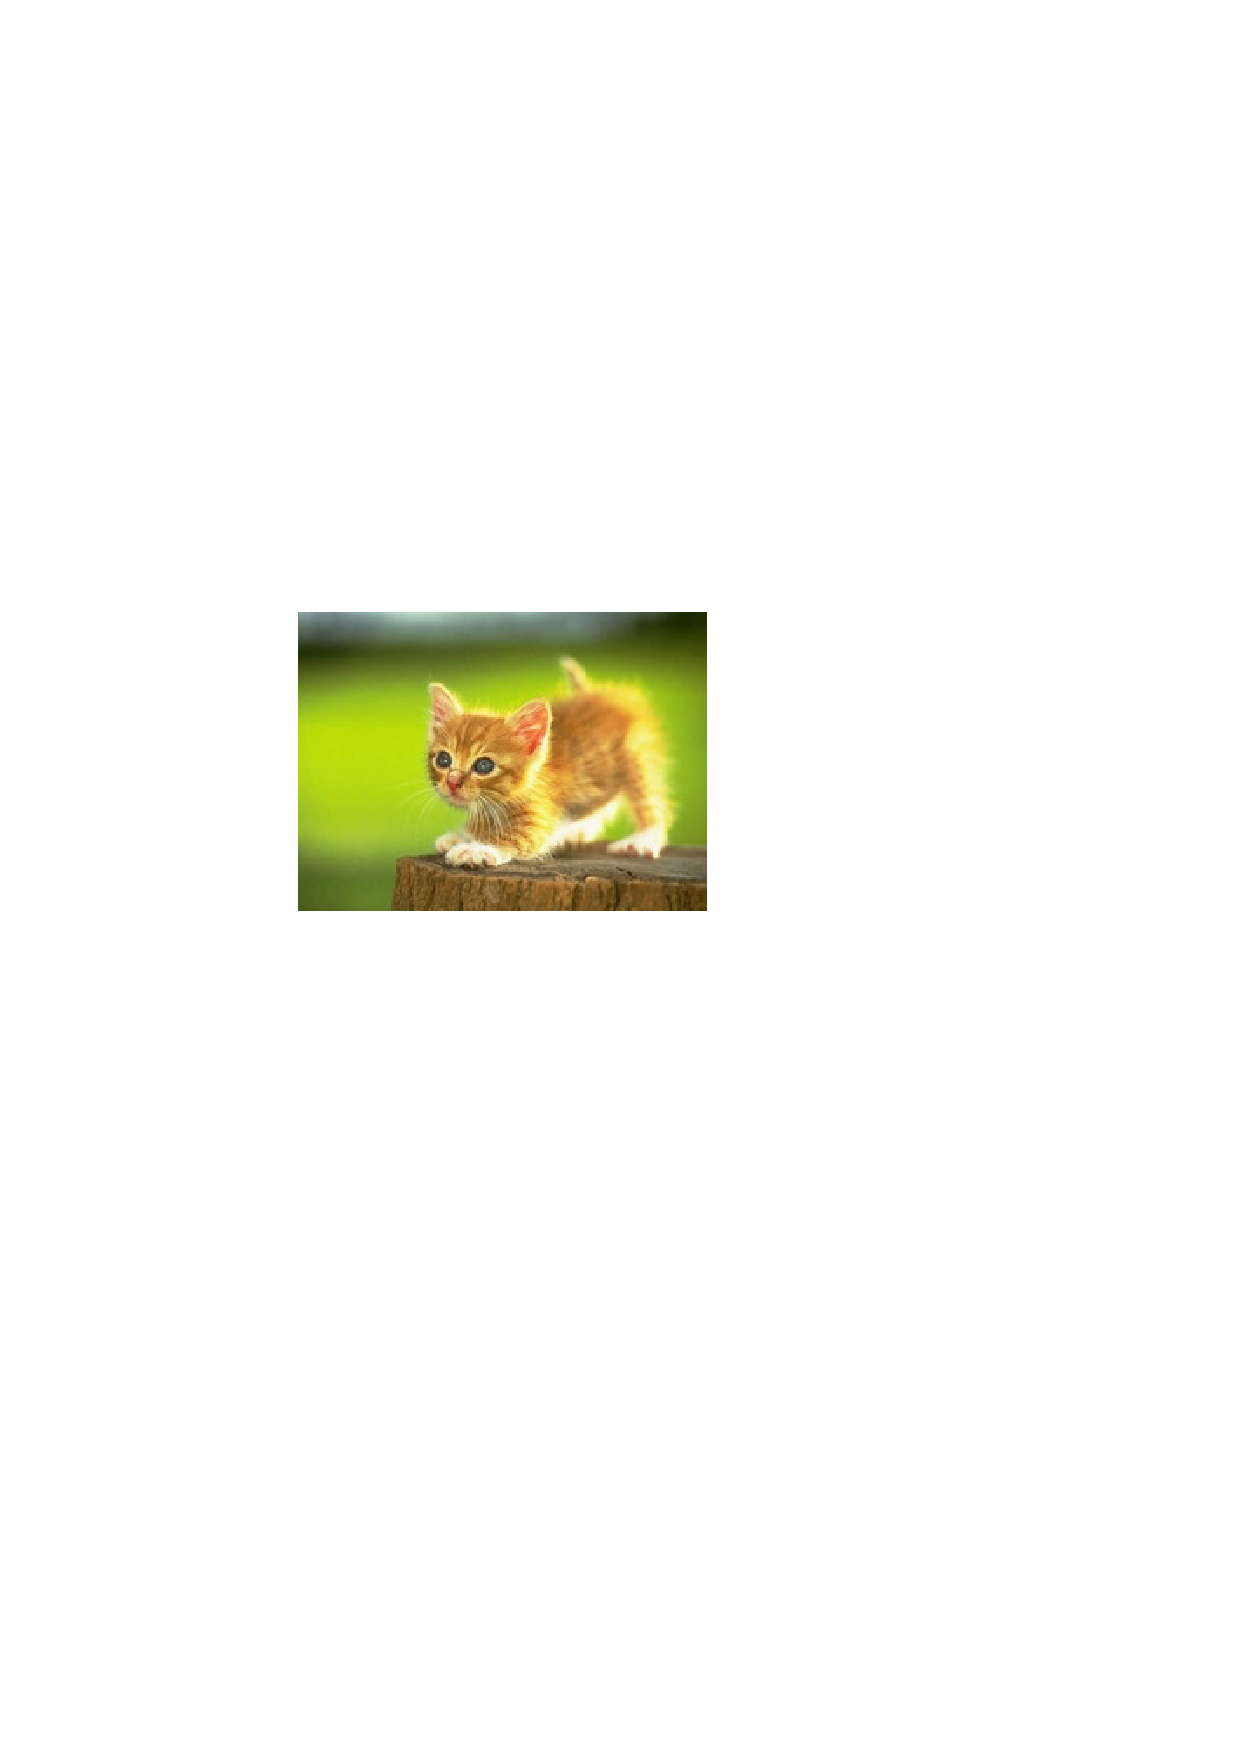
\includegraphics[width=.4\textwidth]{fig/fig-example.pdf}
\caption{一个图片}\label{fig:1}
\end{figure}

\begin{figure}[!h]
\centering
  \begin{subfigure}[b]{0.3\textwidth}
  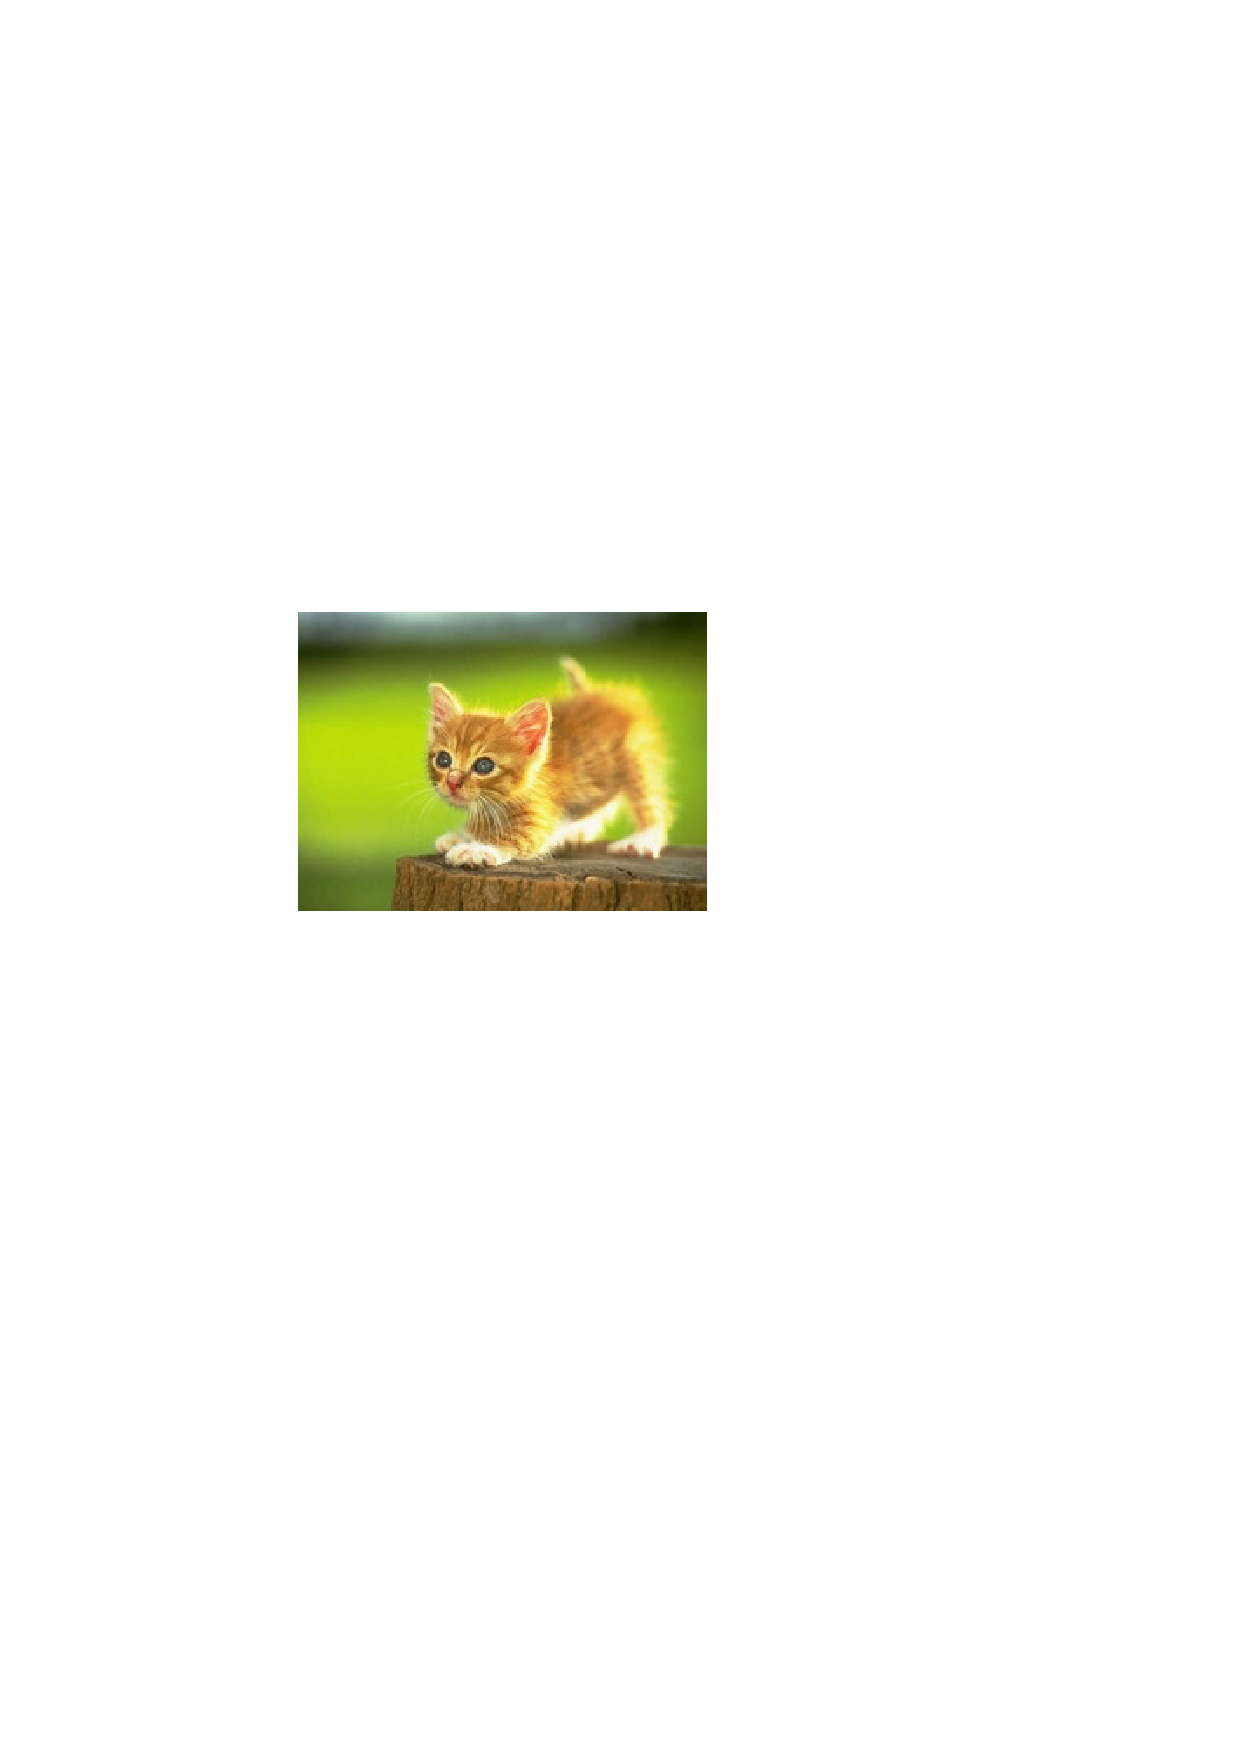
\includegraphics[width=\textwidth]{fig/fig-example.pdf}
  \caption{图片1}\label{fig:2-1}
  \end{subfigure}
  ~
  \begin{subfigure}[b]{0.3\textwidth}
  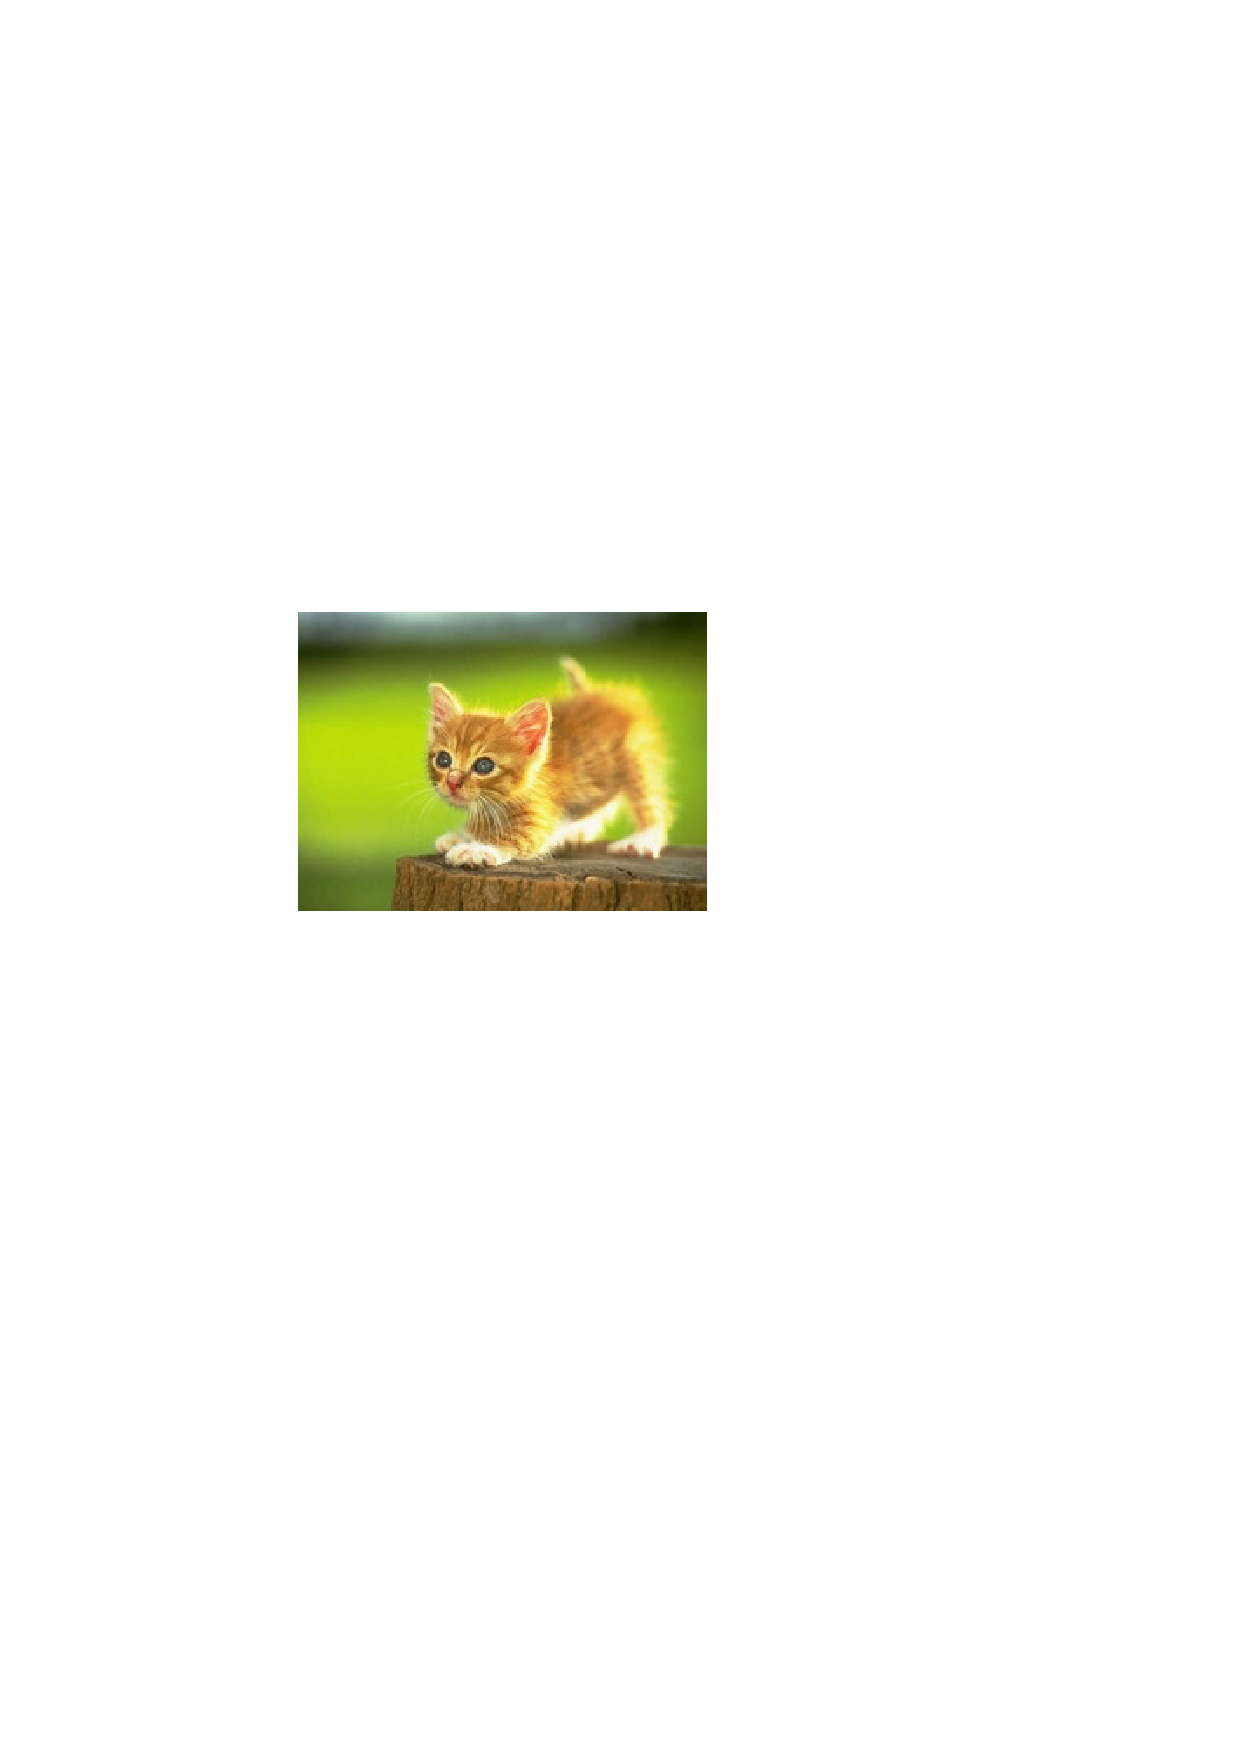
\includegraphics[width=\textwidth]{fig/fig-example.pdf}
  \caption{图片2}\label{fig:2-2}
  \end{subfigure}
\caption{多个图片}\label{fig:2}
\end{figure}

\section{参考文献示例}
这是一篇中文参考文献\cite{Padilla2011};这是一篇英文参考文献\cite{Padilla2011};同时引用\cite{Padilla2011}。

\section[\textbackslash{}autoref 测试]{\texttt{\textbackslash{}autoref} 测试}

\begin{description}
  \item[公式] \autoref{eq:1}
  \item[脚注] \autoref{footnote:1}
  \item[项] \autoref{item:1},\autoref{item:2},\autoref{item:3}
  \item[图] \autoref{fig:1}
  \item[表] \autoref{tab:1}
  \item[附录] \autoref{appendix:1}
  \item[章] \autoref{chapter:Introduction}
  \item[小节] \autoref{sec:pt},\autoref{sec:pd},\autoref{sec:st}
  \item[算法] \autoref{alg:1},\autoref{alg_line:1}
  \item[证明环境] \autoref{def:1},\autoref{proposition:1},\autoref{axiom:1},\autoref{lemma:1},\autoref{theorem:1},\autoref{proof:1}
\end{description}

\backmatter

\begin{ack}
致谢正文。
\end{ack}

\bibliography{bib/bibliography.bib}

\appendix

\begin{publications}
    \item 论文1
    \item 论文2
\end{publications}

\chapter{这是一个附录}\label{appendix:1}
附录正文。


\end{document}

\endinput
%%
%% End of file `thesis.tex'.
